\documentclass{beamer}

% Theme
\usetheme{Madrid}
\usepackage{hyperref}
\hypersetup{
	colorlinks=false,
	linkcolor=blue,
	filecolor=blue,      
	urlcolor=blue,
}
\usepackage{pdfpages}
\usepackage{graphicx}
\usepackage{natbib}
\usepackage{lipsum}
\usepackage{arydshln}
\def\boxit#1{%
	\smash{\color{red}\fboxrule=1pt\relax\fboxsep=2pt\relax%
		\llap{\rlap{\fbox{\vphantom{0}\makebox[#1]{}}}~}}\ignorespaces
}
\renewcommand{\today}{\ifcase \month \or January\or February\or March\or %
	April\or May \or June\or July\or August\or September\or October\or November\or %
	December\fi, \number \year} 




% \AtBeginSection[]
% {
% 	\begin{frame}{Table of Contents}
% 		% \scriptsize
% 			\tableofcontents[hideallsubsections,hideothersubsections,currentsection]
% 	\end{frame}
% }	

% Title page
\title[Monetary Policy
Transmission]{Discussion of\\ \textbf{Bank Market Power and Monetary Policy Transmission: Evidence from Structural Estimation}}
\subtitle{Wang, Whited, Wu, and Xiao (2022, JF)}
\author[Morteza, Najmeh]{Morteza Aghajanzadeh, Najmeh Hajimirza}
\institute[HH Finance]{Households Finance}
\date{\today}

\begin{document}

\begin{frame}
    \titlepage
\end{frame}

% \begin{frame}{Outline}
%     \tableofcontents
% \end{frame}

\section{Introduction}

\begin{frame}{Overview}
    \textbf{How does monetary policy affect bank lending?}\\
    \begin{enumerate}
        \item Reserves channel \citep{bernanke1988credit}
        \begin{itemize}
            \item higher rates $\rightarrow$ higher reserves cost $\rightarrow$ shrinks (reservable) Deposit
        \end{itemize}
        \item Bank capital channel \citep{bolton2000equity}
        \begin{itemize}
            \item duration mismatch $\rightarrow$ higher rates $\rightarrow$ reduce scarce equity capital $\rightarrow$ reduce lending
        \end{itemize}
        \item Deposit channel \citep{drechsler2017deposits}
        \begin{itemize}
            \item banks have market power $\rightarrow$ higher rate $\rightarrow$ keep deposit rate unchanged $\rightarrow$ lower deposit supply $\rightarrow$ lower lending
        \end{itemize}
    \end{enumerate}
    \vspace{0.5cm}
    \textbf{This paper:} 
    \begin{enumerate}
        \item Build and estimate a model with all three channels
        \item \textbf{Finding:} Deposit channel is the most important channel, followed by the capital channel, and then the reserves channel
    \end{enumerate}
\end{frame}
% \begin{frame}{The Deposits channel}
    
    

% \end{frame}

\section{Methodology}

\begin{frame}{Methodology}
    Of course Structural Estimation!\\
    \vspace{0.5cm}
    \begin{enumerate}
        \item Estimate deposit and loan demand curves using BLP framework \citep{BLP1995}
        \item Plug demand curves into a banks' optimization problem (They have 6 representative banks)
        \item Estimate the model using SMD
        \item Examine the counterfactual by removing each channel
    \end{enumerate}
\end{frame}

\section{Comments}
\begin{frame}{Comments}
    \begin{enumerate}
        \item \textbf{Missing channel} 
        \item \textbf{External validity}
        \item \textbf{Counterfactuals} 
    \end{enumerate}    
\end{frame}
\begin{frame}{Missing channel}
\begin{figure}[htbp]
    \centering
    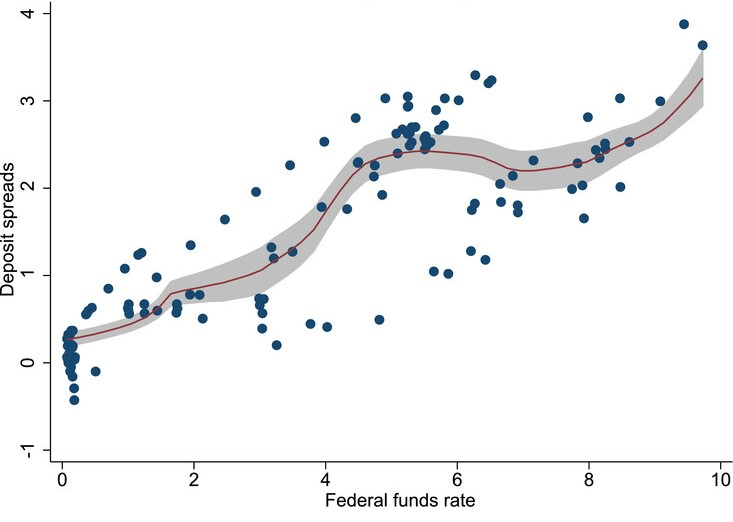
\includegraphics[width=0.45\textwidth]{Figure1a.jpg}
    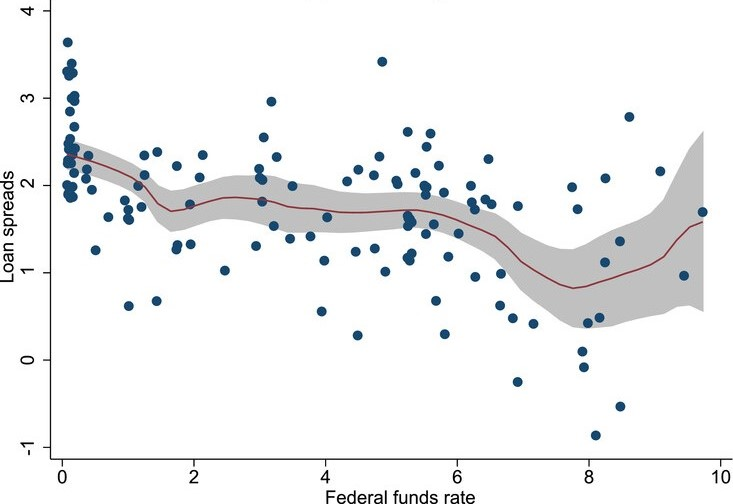
\includegraphics[width=0.45\textwidth]{Figure1b.jpg}
\end{figure}
\end{frame}

\begin{frame}{External validity}
    \begin{figure}[htbp]
        \centering
        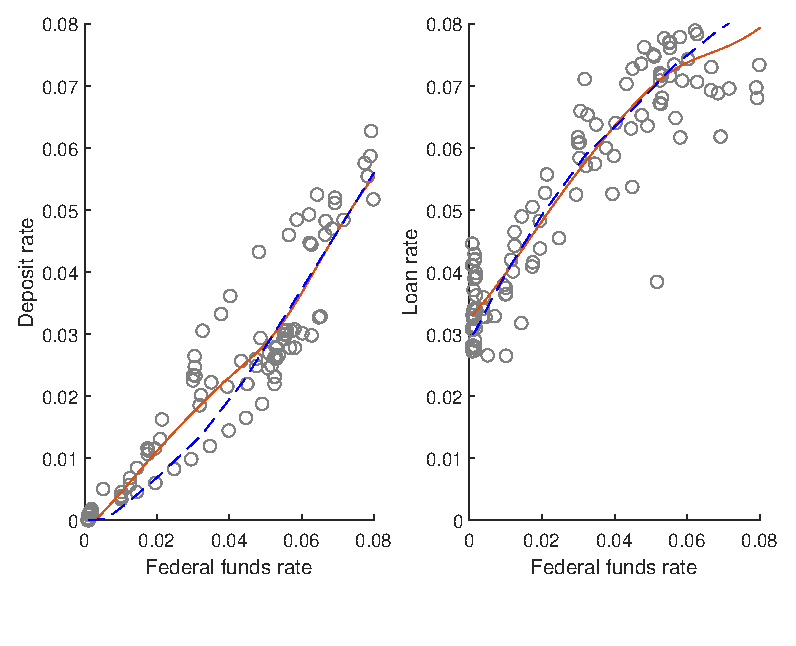
\includegraphics[width=0.7\textwidth]{replication_figure3.eps}
    \end{figure}
\end{frame}

\begin{frame}{External validity}{Replication}
    \begin{figure}[htbp]
        \centering
        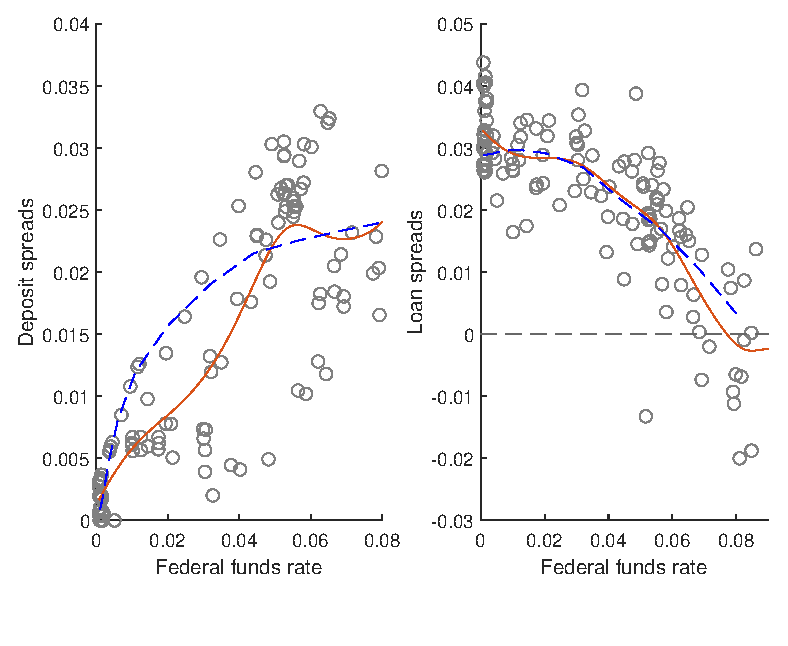
\includegraphics[width=0.7\textwidth]{replication_figure1.eps}
    \end{figure}
\end{frame}

\begin{frame}{External validity}
    \begin{figure}[htbp]
        \centering
        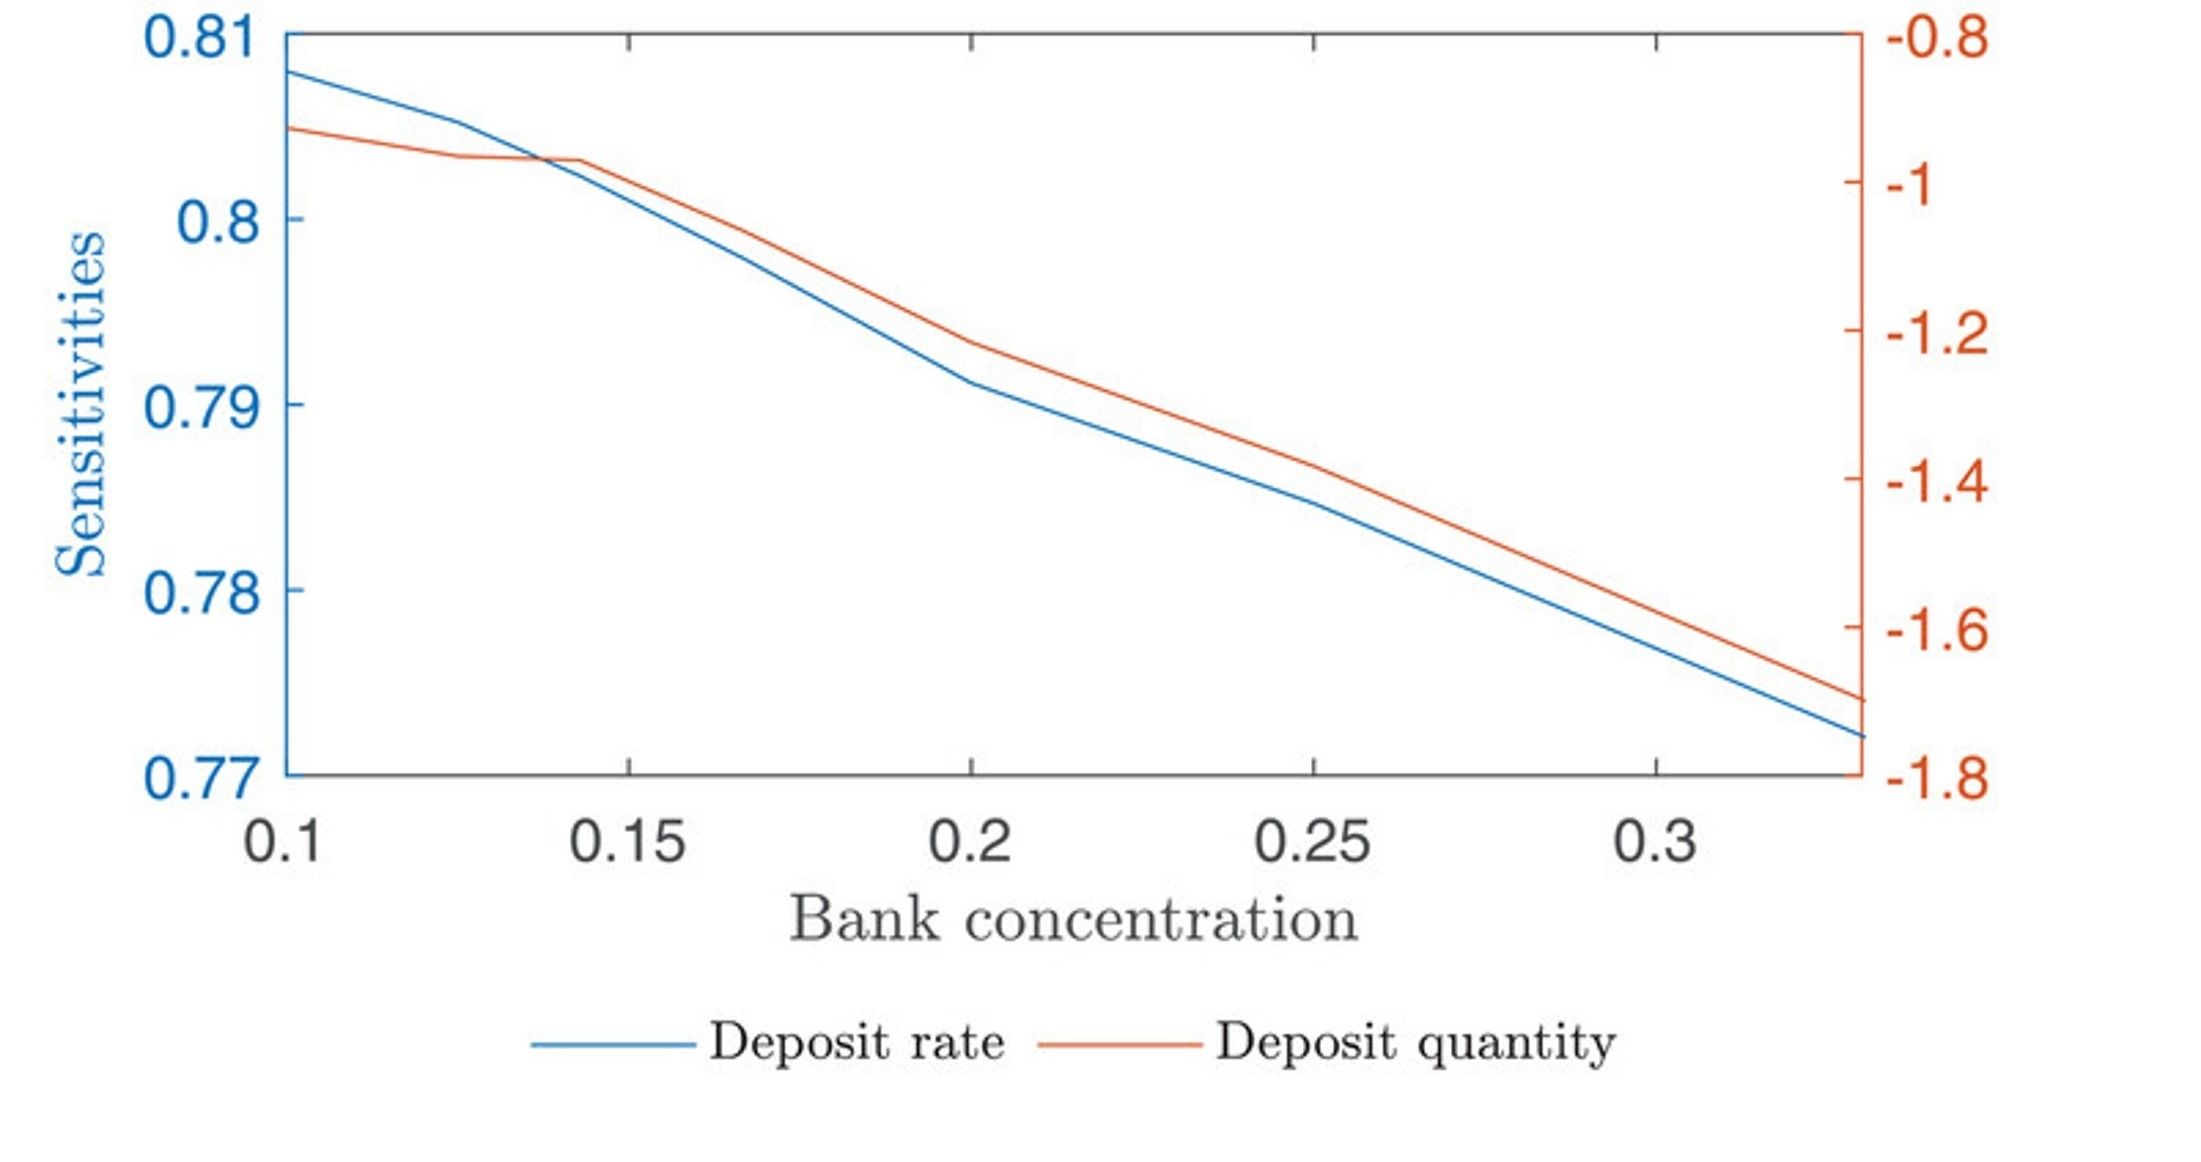
\includegraphics[width=0.45\textwidth]{Figure4a.jpg}
        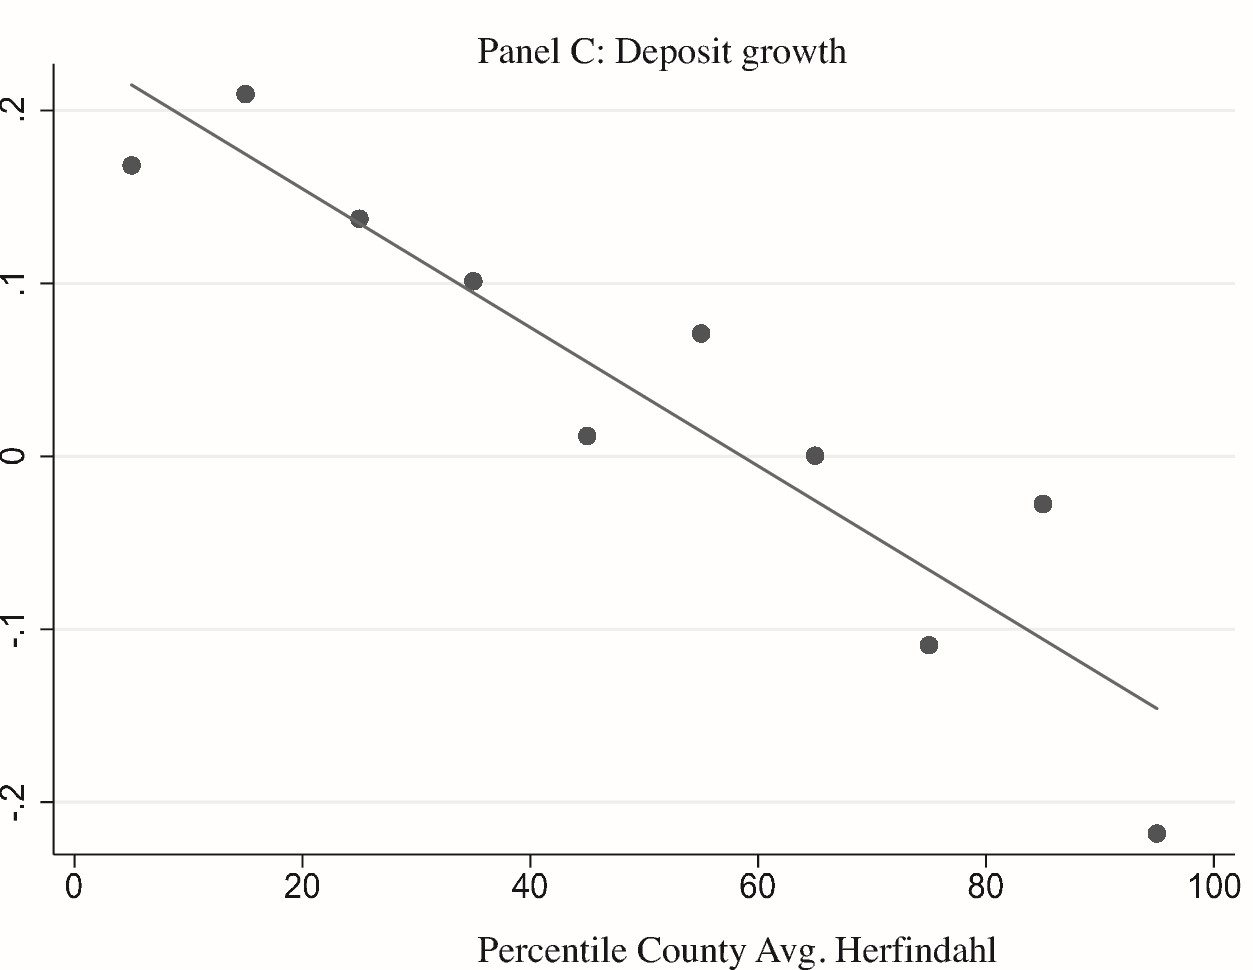
\includegraphics[width=0.45\textwidth]{DSS2017.jpg}
        \end{figure}
\end{frame}

\begin{frame}{Counterfactuals}

    \begin{table}
        \resizebox{.8\textwidth}{!}{\begin{tabular}{clcc}
            \hline
             &  & Sensitivity & Change (\%) \\
            \hline
            (1) & All frictions & $-1.641$ & - \\
            (2) & - Reserve regulation &$-1.499$ & $8.65\%$ \\
            (3) & - Capital regulation & $-1.248$ & $23.91\%$ \\
            (4) & - Deposit market power & $-1.132$ & $31.00\%$ \\
            (5) & - Loan market power & $-1.951$ & $-18.91\%$ \\[1ex]
            \cdashline{1-4} \\[-2ex]
            (6) & Only Loan market power & $-0.913$ & $44.36\%$ \\
            (7) & Only Deposit market power & $-1.951$ & $-18.88\%$ \\
            (8) & No frictions & ? & ? \\
            % (8) & No frictions & $-2.461$ & $-50 \%$ \\
        \end{tabular}}
    \end{table}
\end{frame}

\section{Conclusion}
\begin{frame}{Conclusion}
    \begin{enumerate}
        \item This paper builds and estimates a model with all three channels: deposit, capital, and reserves. And the deposit channel is found to be the most important channel
        % \item The methodology used in this paper involves estimating deposit and loan demand curves using the BLP framework, plugging demand curves into a banks' optimization problem, estimating the model using SMD, and examining the counterfactual by removing each channel.
        \item The missing channel in this paper is the risk taking behavior of banks, which could be an interesting avenue for future research.
        \item The external validity of the model is not fully supported by replication results and comparison with other studies.
        \item The paper needed to provide more details on the counterfactuals. For example, how much of the deposit channel is due to the deposit market power and how much is due to the loan market power?
    \end{enumerate}
\end{frame}


\scriptsize 
\begin{frame}[allowframebreaks]{References}
    \bibliographystyle{aea}
    \bibliography{ref.bib}
\end{frame}
	
\normalsize
\end{document}



\scriptsize 
	\begin{frame}[allowframebreaks]{References}
			\bibliographystyle{aea}
\bibliography{ref.bib}
		
	\end{frame}
	
	\normalsize
\end{document}
